\documentclass[]{article}
\usepackage{hyperref}
\usepackage{algorithm}
\usepackage[noend]{algpseudocode}
\usepackage{amsmath}
\usepackage{amssymb}
\usepackage{graphicx}
\usepackage{subfig}
\graphicspath{ {./figures/} }


\newcommand*{\QEDA}{\hfill\ensuremath{\blacksquare}}%
\newcommand*{\QEDB}{\hfill\ensuremath{\square}}%

\makeatletter
\def\BState{\State\hskip-\ALG@thistlm}
\makeatother

\begin{document}

\title{}
\author{}

\maketitle
\begin{abstract}
Summary Of The Problem
\end{abstract}
\section{Introduction}

\section{Literary Review}
\paragraph{}
As we approach the limit of De Morgan's law, we come to an age in computing where sequential computing is limited by processing speed. Using RAM (Random Access Memory) as our base model of computation we create optimal sequential algorithms. However, in the age of big data, these sequential algorithms are not powerful enough to process all the data in reasonable time. Thus, we turn to parallel computing to where we have two models of computation which attempt to divide work. The first model assumes that all knowledge is known about the problem, then divides work base accordingly; this is known as the field of parallel computing. The second approach assumes that only local information is known about the problem, and through a series of steps, protocol definitions, and message passing an answer can be derived/approximated; this is known as the field of distributed computing. However, there are tradeoffs to both approaches like : speed, run-time, correctness, optimality. Most algorithms take a tradeoff between these two fields as computation gets further away from processors.

\paragraph{}
In this age being able to extract information form graphs becomes more prevalent in analyzation of web link graphs, social networks, and many other graphs types. One property that we can extract is graph connectivity. In graph theory graph connectivity is the minimum number of vertices, or elements that need to be removed to separate nodes into isolated subgraphs [7]. A very similar definition of this is the minimum cut of a graph where a minimum cut is defined as the minimum partition of verticies, and edges into two disjoint sets. For simple unweighted graphs David R. Krager et al [8] created a randomized sequential algorithm based on properties preserved when edge contraction is applied. The papers by David R. Krage et al [9], and Barbara Geissmann et al. [10] further improve the algorithm by adding parallelisation. The downside of parallel algorithms introduced is that they are still based on the Parallel Random Access Memory (PRAM) model which can be used to prove theoretical bounds on algorithm. But the algorithms introduced disregarded hardware limitations where CPU cache is finite, and message passing to start up threads/processes are costly. It is noted that the paper in Barbara Geissmann et al. [10] attempts to improve cache misses by creating monotonic sequences to be read, however, the paper still relies heavily on parallelism of
 subroutines.
 
 \paragraph{}
 Another version of this problem comes from weighted undirected graphs. The goal is to find a cut where the sum of the edge weights are minimum. The Stoer-Wagner algorithm by Mechthid Stoer et al. [11]  is a good sequential recursive algorithm for solving undirected weighted graphs with non-negative weights in $O(|V||E|+|V|^2\log|V|)$ time. Usually the min-cut with respect to weighted undirected graphs is linked with the maximum flow problem as the minimum cut is often the bottleneck of the network [12,13].
 
 \paragraph{}
 A subfield of graph connectivity is connected components. Connected components can be divided into two categories: strongly connected components (SCC), and weakly connected components (WCC). A graph is said to be strongly connected if every vertex is reachable from every other vertex. Then a SCC is the same definition, but the maximal subgraph that keeps this property. The SCCs of a directed graph form partitions of subgraphs where they themselves are strongly connected. WCCs of a directed graph form a subgraph for every pair in the subgraph there exists a path, but not necessarily a bijective path. 
 
 
 
 \paragraph{}
 One of the earliest algorithms introduced is Tarjan's algorithm which uses the properties of depth first search (DFS) to find SCC given by Robert Tarjan [16]. Later  Edsger W. Dikstra came up with the path-based strong component algorithm seen in [17]. A simpler algorithm was also found after named Kosaraju's algorithm and published by Micha Sharir [17]. However, all of these algorithms abuse depth first search to find SCC, yet for parallel algorithms DFS is hard to paralyze. In fact, it was proved by John H. Reif that DFS is P-complete [19]. Therefore parallel algorithms do not focus on DFS when computing strongly connected components seen in Lisa K. Fleischer et al. [20], and Sungpack Hong et al. [15].
 
 \paragraph{}
 There is another version of Connected Components in undirected graphs. Unlike the directed version, if there is a path, then that path is a SCC since edges are bidirectional. Therefore the undirected version of SCC focuses on finding disjoint subgraphs in the original graph, since each disjoint subgraph is itself a SCC of the original graph. One may also relate this to finding WCC in a directed graph, since a path represents a bijective edge in undirected graphs. However, by doing so the WCC may contain a SCC in the original graph. A simple sequential algorithm can be done to find this where you take a DFS, or a breadth first search (BFS). Once you have exhausted your search, you select a non-traversed vertex to find the next SCC [21]. There have also been algorithms for dynamically changing graphs researched by Yossi Shiloach et al. [22].
 
 \paragraph{}
 As graphs increase in size, so does the amount of processing power required. In the field of SCC on undirected graphs there have been several subfields in which parallelization has taken affect.  The first parallel algorithms dealing with SCC on undirected graphs deal with spanning forests [23,24,25,26,27,28,29,30,31,32,33,34,35,36,37]. The algorithms by Uzi Vishkin et al. [36,4], and Awerbuch et al. [37] work by combining vertices into trees, such that a constant number of vertices are deleted every iteration, but does not guarantee a constant fraction of edges. Thus they require $O(|E| log |V|)$ work. The random algorithm by Reif, and Phillips [?] work by contracting vertices in the same component, which guarantees a constant number of vertices every iteration, however, it again does not guarantee a constant fraction of edges. Thus the expected work is $O(|E| log |V|)$.
 
 \paragraph{}
 Work-efficient polylogarithmic-depth parallel connectivity algorithms have been designed in theory [38,39,40,41,42,43]. These algorithms are based on random edge sampling, or filtering edges. However, these have complicated structures which may be impractical to implement in practice. 
 
 \paragraph{Min-Label Propagation}
 \paragraph{BFS-CC}
 
 \paragraph{}
The algorithm which we will be focusing on is based on Shilovach-Vishkin[4] which has $O(\log n)$ parrallism, an uses a maximum of $2|E| + |V|$ processors. Shilovach-Vishkin represent their CC as a forest where each tree represents a connected component. They have two key phases \textit{hook}, and \textit{shortcut}. \textit{Hook} is reponsible for connecting processed components together where it hooks new nodes with their respective component, or connectes two componnets together given the current knoldge know of the graph. They prove that this process results in tree that have height at most $\lfloor\log_{3/2}n\rfloor + 2$. The \textit{shortcut} phase results in a compression of the trees in the forest such that they have depth at most one. 


 
 \section{Statment of Problem}
\paragraph{}
The key problem with Vishkin-Shilovach is that work was done on a per-node basis, such that there may be duplicate reads to the same edge. Furthermore, if there is a large component in the graph, then the algorithm would read all edges that exist within that component. Thus, if we have a large complete graph, then all $|E|=|V|^2$ edges in this complete graph would be traversed, when only $|V|$ edges are needed inorder to determine a CC.

\paragraph{}
A solution to this is to sample for the largest component in the graph, and skip any node not processed in this component.
This algorithm was proposed by Michael Sutton et al.[1] where they attempt to do superlinear work on the number of edges in the graph, such that no edges are visited twice. The algorith that they present is called \textit{afforest}, which is similar in nature to the algorithm presented by Shilovach-Vishkin. We will be performing a review on \textit{afforest} guaging performace, and filling in missing proofs not fully described in the original paper.


 - state research question : to analyze the performance of afforest\\
 - why question is answered\\
 - discussion why this question is worthwhile\\
 
 \section*{Afforest}
 \paragraph{}
 Similar to Shilovach-Vishkin, afforest's underlying data structre is a forest. In this forest each tree is represented as a connected component found thus far in the view of the processed graph. For all $v\in V$, $v$ has a unique identifier. We denote the symbol $\pi(v)$ to represent the parent of $v$, such that we hold an invariant inwhich $\pi(v)\le v$. We note that if $v$ is the root then $\pi(v) = v$.
 
 \paragraph{}
 The basis of afforest is contingent on two operations : link, and compress. Link is seen in Algorithm 1. Link ensures that two verticies will be in the same component tree. Link searches the tree(s) for a root with the larger identifier. Upon finding the root with a larger identifier link attempts a Compare and Swap (CAS) opeartion inorder to connect the larger tree to the smallar identifier. The smallar identifier does not nessarily need to be the root of the tree. We can see that our invarient still holds.
 
 
  
\begin{algorithm}
\caption{Link Operation}\label{euclid}
\begin{algorithmic}[1]
\Procedure{link}{$edge(u,v)$ , $\pi$}
\State $p_1 \gets \pi(u)$
\State $p_2 \gets \pi(v)$
\While{$p_1 \neq p_2$}
  \State $h \gets max\{p_1,p_2\}$
  \State $h \gets min\{p_1,p_2\}$
  \If {$compare\_and\_swap(\pi(h),h,l)$} \Return
  \EndIf
  \State $p_1 \gets \pi(\pi(h))$
  \State $p_1 \gets \pi(l)$
\EndWhile\label{euclidendwhile}
\EndProcedure
\end{algorithmic}
\end{algorithm}

\begin{figure}[H]%
    \centering
    \subfloat[Case where CAS happens at both roots]{{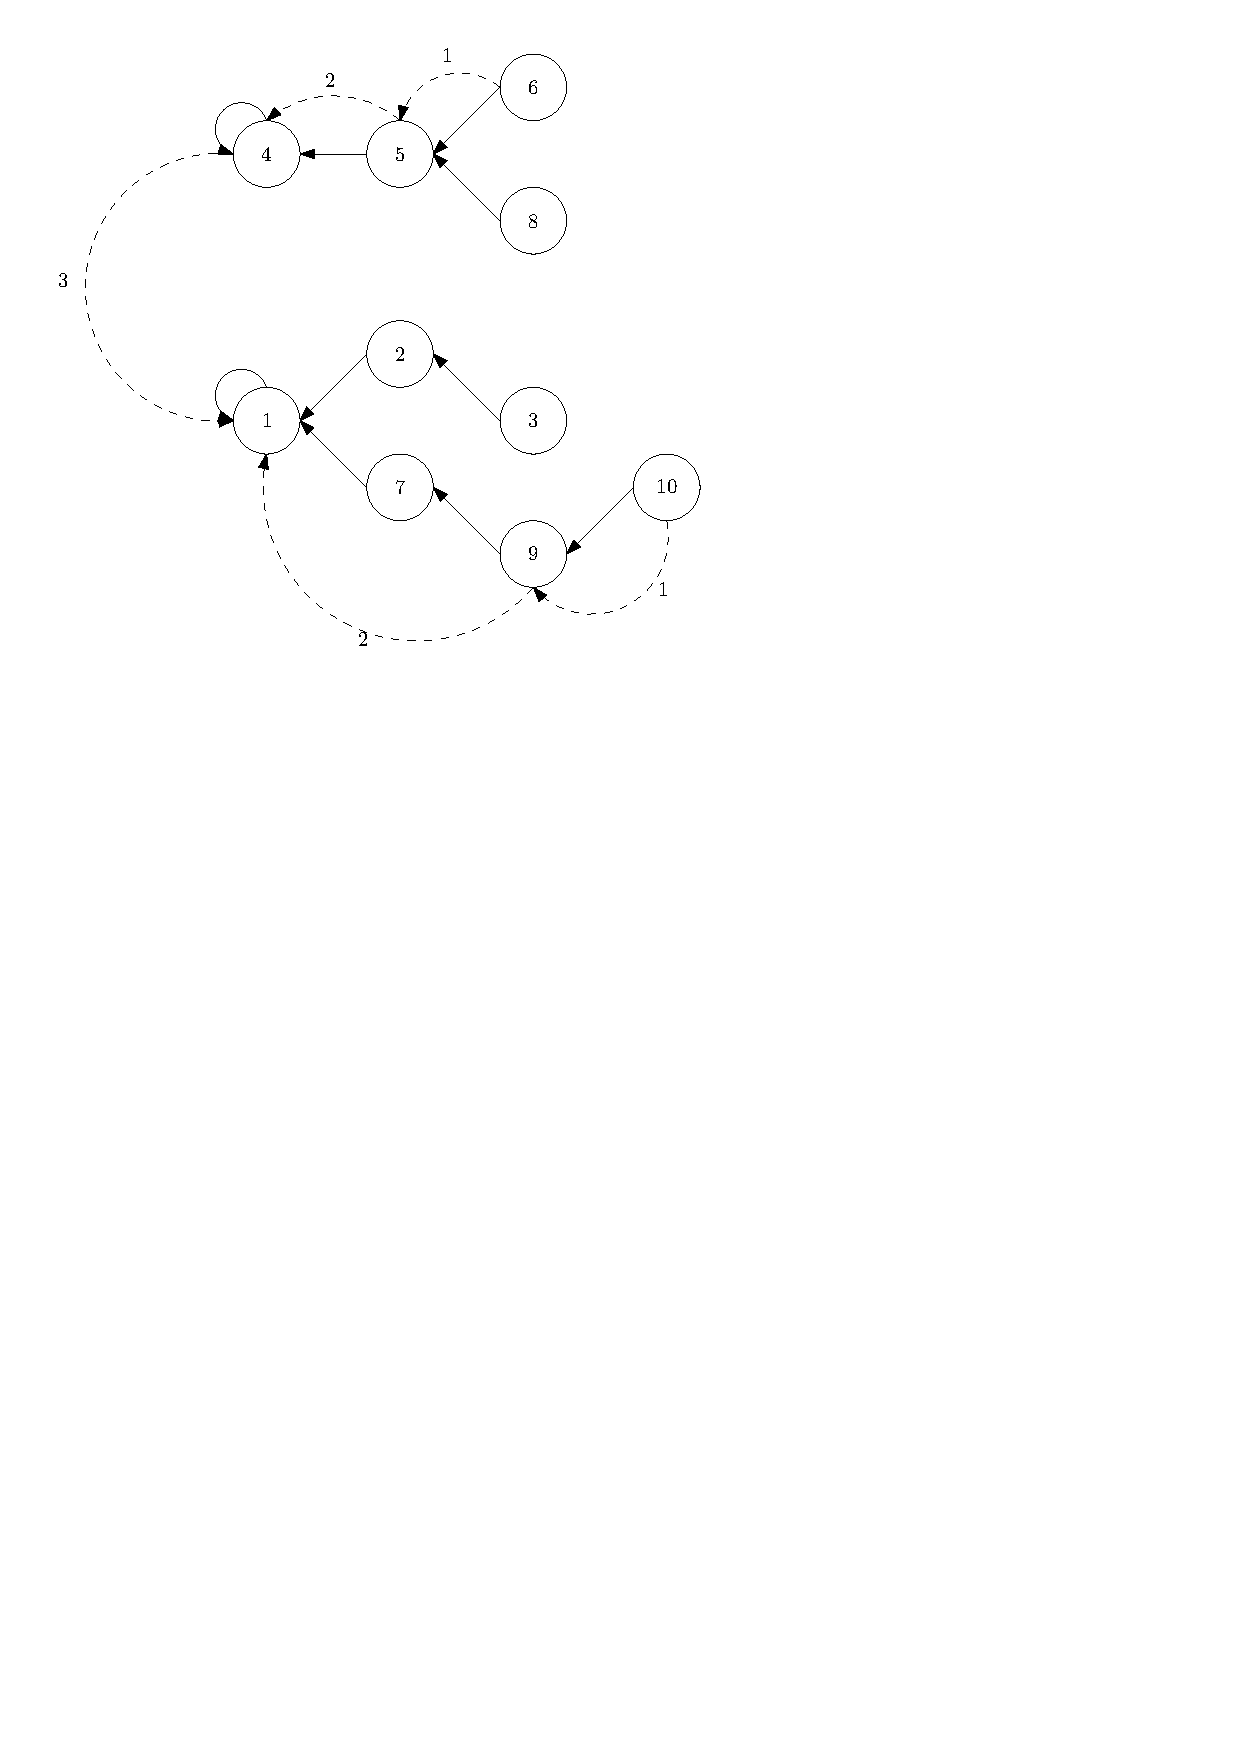
\includegraphics[width=5cm]{fig-1} }}%
    \qquad
    \subfloat[Case where CAS happens at one root]{{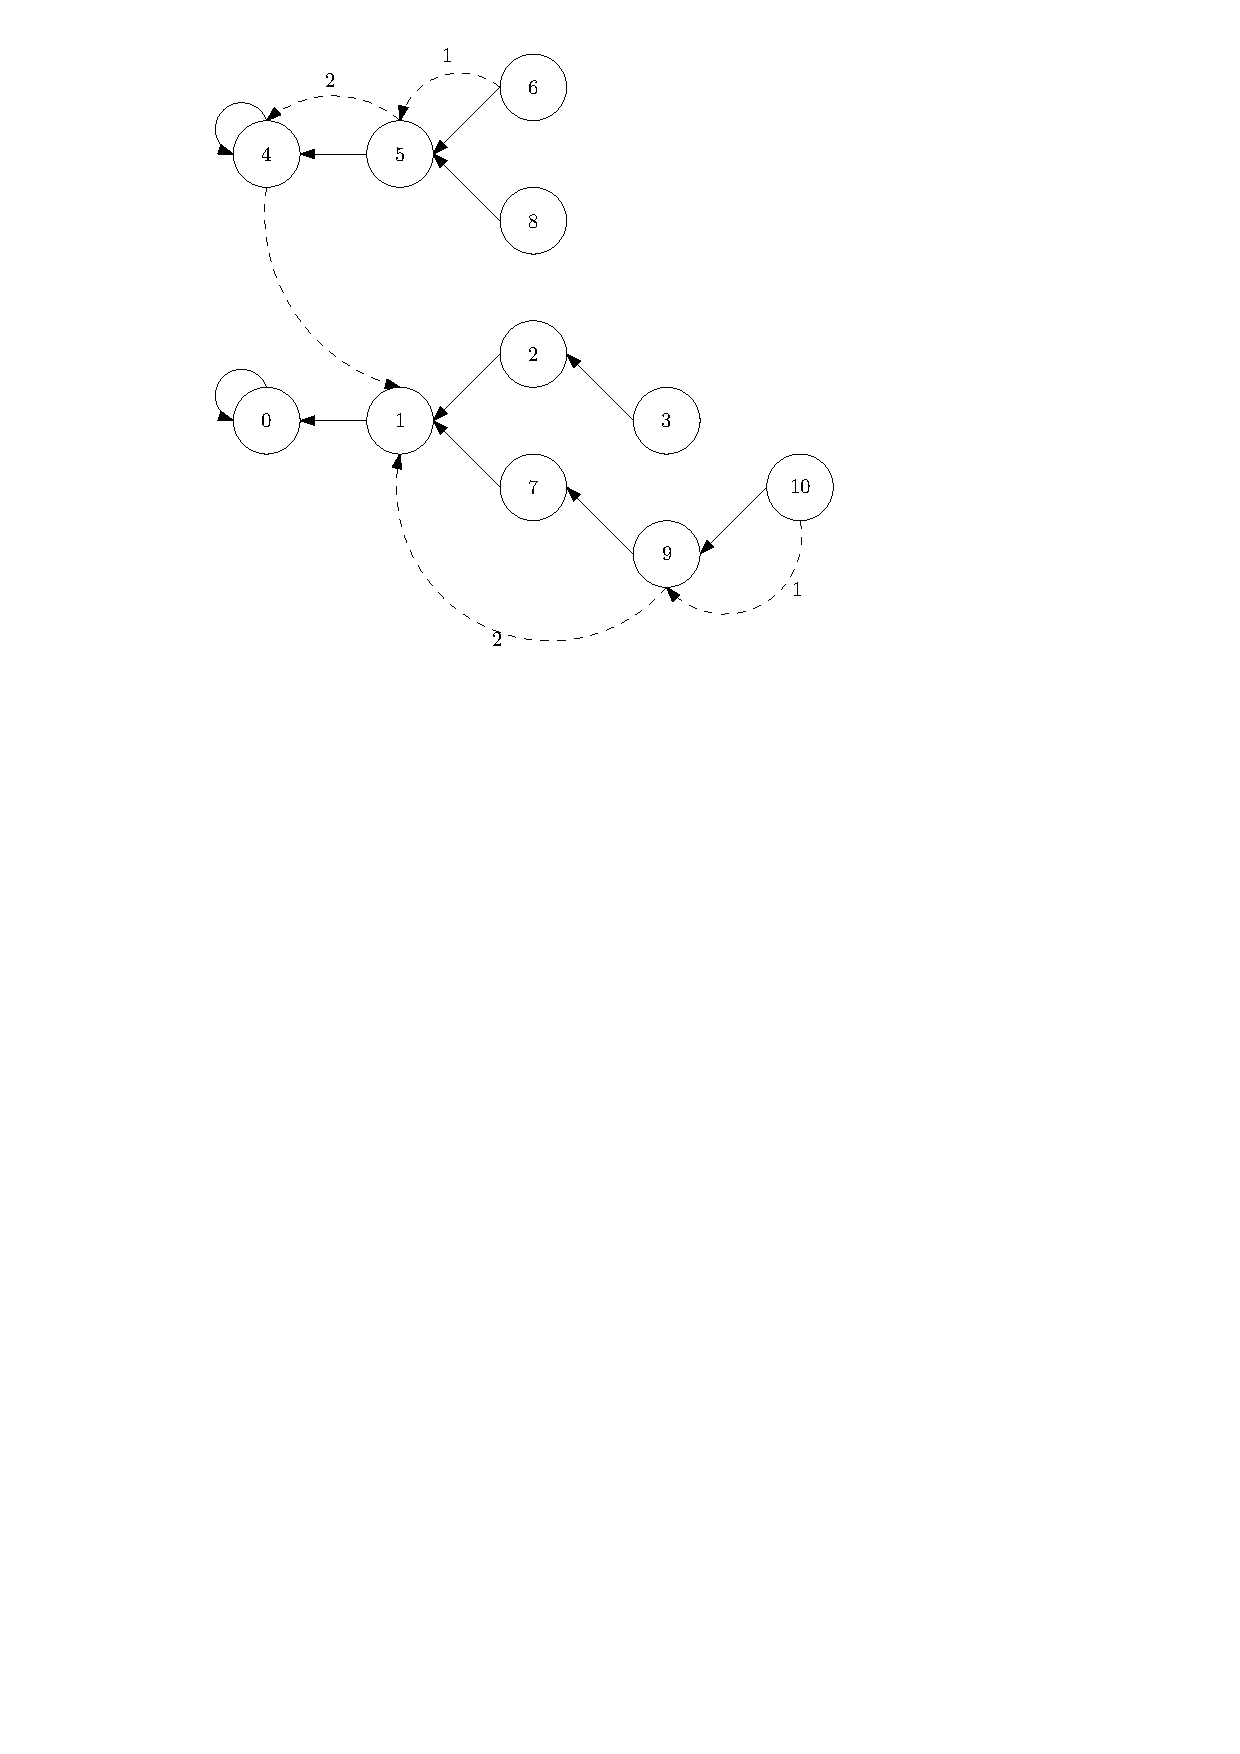
\includegraphics[width=5cm]{fig-2} }}%
    \caption{Link operation traversing up component trees linking edge(6,10)}%
    \label{fig-link}%
\end{figure}
 
  \paragraph{}
In figure \ref{fig-link}, we see the opeation of adding the edge with $u=6$, and $v=10$. We see that in both cases we traverse up to the largest root $4$, and we connect the tree rooted at $4$, to the tree rooted at $1$. It can be seen that not matter where we connect root $4$, there is always a path from from every element in the tree rooted at $4$ to the new component tree root $1$.



 \paragraph{Lemma 1.}
 If the endpoints of link $u$, and $v$ are within the same component tree, then the ancestors of the component tree do not change. Since a CAS operation is only triggered when the largest node is the root, and since our invarient proves that the root is the smallest value in the tree, the CAS opeartion is never triggured.
\QEDA 
\paragraph{Lemma 2.}
If the endpoints of link $u$, and $v$ are not within the same component tree, then the link operaiton will ensure that both trees are merged into one component tree. There are three possible cases that we need to conver to prove this.

\begin{enumerate}
  \item If the processors' $h$ remains the root, and CAS succeds, then we know that $h$, and $l$ are directly connected. Resulting in one connected component
  \item If another processor connecets $h$ to the tree, then we apply lemma 1. This results in one connected component.
  \item If another processor connecets $h$ to $l'$ such that $l'$ does not live in the tree of $u$, nor the tree of $v$. Then $h \neq \pi(h)$. We then repeat searching up the tree, and we end up with the same problem as decribed in Lemma 2. Since there are a finite number of vertecies, then there are also a finite number of components. Therefore the operation will complete results in one connected component containing both $u$ and $v$.
\end{enumerate}
\QEDA
\paragraph{Lemma 3.}
If we apply link to all edges, then the resulting component tree represents the CC of the original graph. $\forall edges(u,v)$, $u$ and $v$ will be in the same component since we apply link to all edges. Then by Lemmas' 2, and 3 all edge pairs will be in the same component.

\paragraph{}
By defenition a CC is connected if there exists a path between all pairs in the component. If we take one such path $x_1,x_2,...x_{n-1},x_n$ then link would be applied to : $(x_1,x_2),...,(x_{n-1},x_n)$. Which means all the nodes in the path will be in the component tree. If we take take the set of all paths and convert it to the set of all edges, then every vertex that is an element of a CC $C_i$, is also an element of a unique component tree coresponding $C_i$. Since we apply link to all edges, then we cover the set of all possible paths. Therefore the a resulting component tree represents a connected component in the original graph.
\QEDA

\paragraph{}
The second most important opeartion of afforest is the \textit{compress} opeation seen in Algorithm 2.
Compress makes a single node search for the root of its component tree. If we apply compress to all edges, then this results in a depth one tree. This is seen in figure \ref{fig-compress} where a tree is converted to a depth one tree.

\paragraph{}
A depth one tree is obtained when all nodes apply the compress operation. At each iteration in the while loop a node reduces it's depth by at least one. We say at least one since at any time another processor could be modifying the path, however, any modificaiton to the path results in a shorter path. Once a node has reached the root of the tree we stop, thus create a depth one node. If we apply this to all nodes then all nodes will have depth one.
 
 
 \begin{algorithm}
\caption{Compress Operation}\label{euclid}
\begin{algorithmic}[1]
\Procedure{compress}{$v$ , $\pi$}
\While{$\pi(v) \neq \pi(\pi(v))$}
\State $\pi(v) \gets \pi(\pi(v))$
\EndWhile\label{euclidendwhile}
\EndProcedure
\end{algorithmic}
\end{algorithm}


\begin{figure}[H]%
    \centering
    \subfloat[Before Compress Operation]{{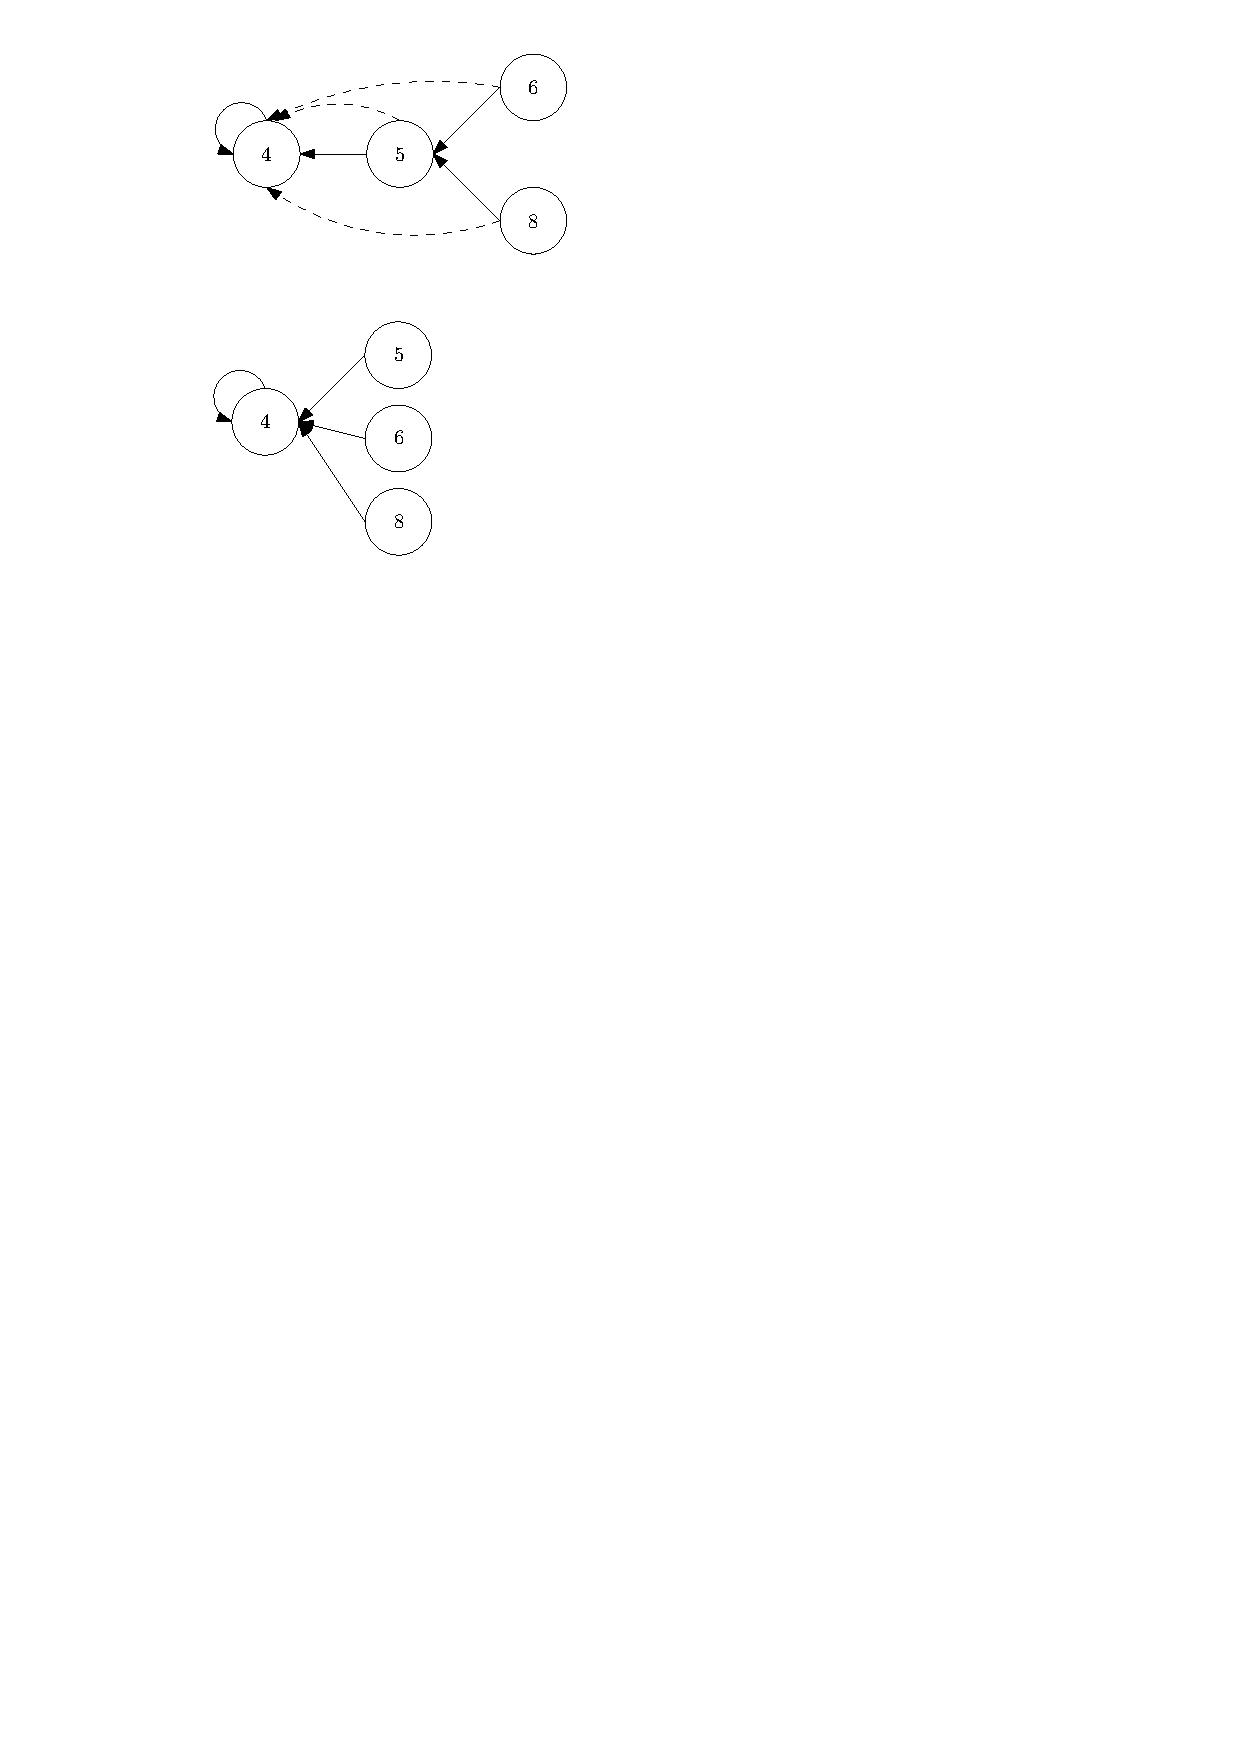
\includegraphics[width=5cm]{fig-3} }}%
    \qquad
    \subfloat[After Compress Operation]{{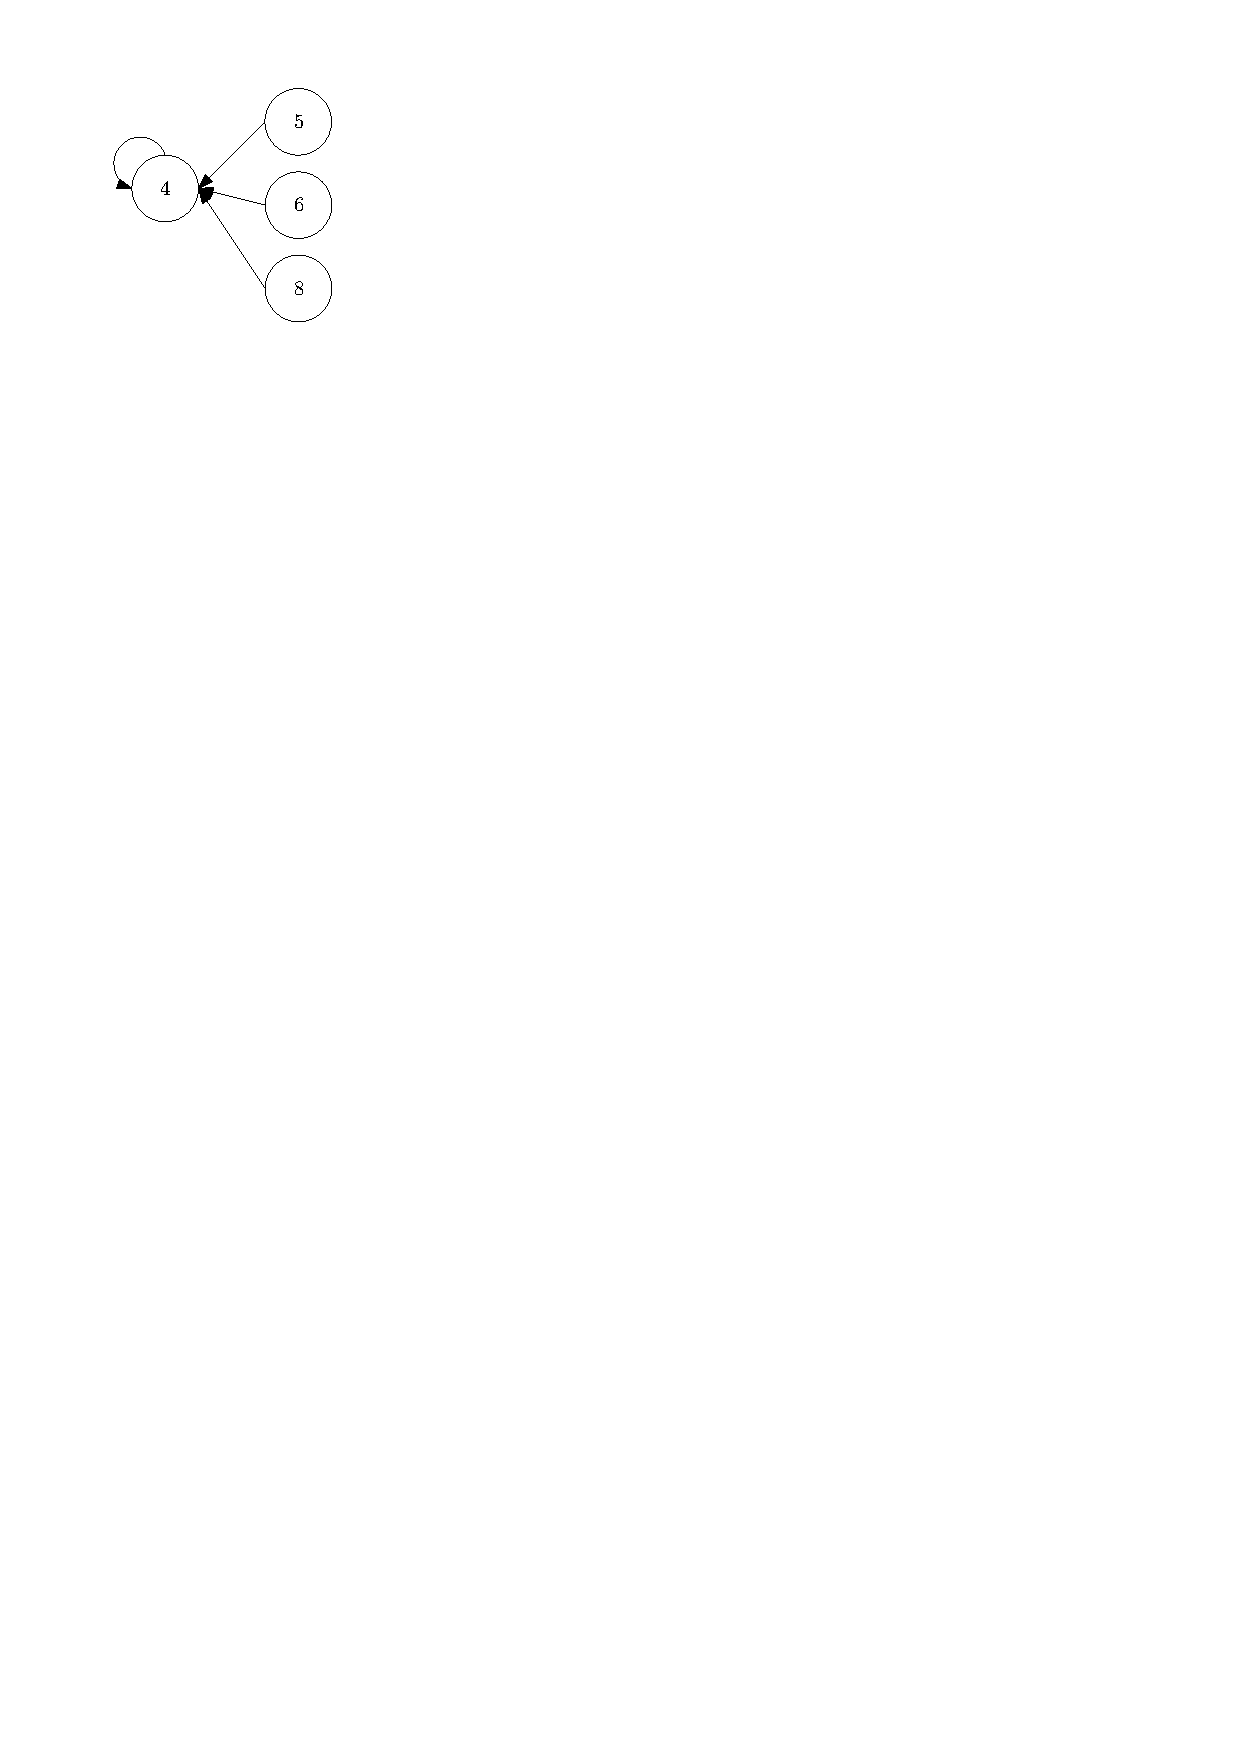
\includegraphics[width=3cm]{fig-5} }}%
    \caption{Example of a Compress Operation}%
    \label{fig-compress}%
\end{figure}
 
 \paragraph{}
 One might notice that we traverse that we may traverse the whole tree in link, and that we may traverse the whole tree in compress.
 This would result in a sequential span of the maximum height of one of these tree. If under the assumption that only the roots of the tree change, we propose an exact expected value for the height of the tree. If our assumption is false, then we still would have obtained a lowerbound on the expected height of the tree. Inorder to prove this we must look at Union-Find data structure invented by Kruskal[60].
 
 \paragraph{}
 Union-Find is an algorithm similar to afforest. The data structure consists of a forest of trees, such that each tree represents components in a union. If we want to find the union of $\{x_1,x_2\}$ then the algorithm finds the root of $x_1$, and the root of $x_2$.
 If the roots are in the same tree then no work is needed to be done since they are in the same set. If the roots are not in the same tree, then smallest root is chosen as the new root of the tree such that the largest root is a child of the smallest root. In other words if $x_1 < x_2$, then set $\pi(x_2) = x_1$. Under the assumption we made that only roots change similar to figure \ref{fig-link} a), then this data structure exhibits the same properties as afforest.
 
 \paragraph{}
 Obviously the worst case results in a tree with length $n$, where $n$ is the number of elements in the set. Therefore let us consider the expected case. First we assume that the addition of union-find requests are uniformily random. Second, we only focus on the largest tree durring formation. By doing so we get an upper bound on the expected height, and we can apply backwards analysis. 

\paragraph{} 
Thus, let $X$ be the height of the largest tree. Let $X_i = 1$ when we pick a node at iteration $i$ that increases the height, and let $X_i=0$ otherwise. There is no bound on the number of iterations, but we choose a bound $n$ as we can form any permutation of sets, thus each iteration results in a union. Now we condider the largest tree $T$. At any iteration $i$, $T$ grows at most by $1$ as we add an edge, or we add a tree which is at most the height of $T$. If we attempt to build our tree with $i=0$, it is hard to count. Therefore, let us consider T at iteration $i$. Between iteration $i$ and $i-1$ we choose one pair out of the $(n-(i))$ possible choices that will increase the height of the tree. Therefore the probility that we choose that pair between one iteration is : $\frac{1\cdot(n-(i+1))!}{(n-i)!} = \frac{(n-i+-1)!}{(n-i)!} = \frac{1}{(n-i)}$. Therefore if we apply this over all iterations then the expected maximum height is :
\begin{align*}
  E(X) = E(\sum_{i=1}^{n}X_i) = \sum_{i=1}^{n}E(X_i) = \sum_{i=1}^{n}\frac{1}{n-i} = \sum_{i=1}^{n}\frac{1}{i} \le Hn(n) \le ln(n) +1
\end{align*}

Therefore we have showed that the expected height is not more than $O(ln(n))$, but how much does this deviate from the expected value.
We can use Markovs Inequality to calculate with high probility that this is true. We assume that $a = {n^{-d}}$, where $d$ is a constant. We can then use Markov's Inequality to prove that :
\begin{align*}
  P(X\ge a) = P(X \ge n^{-d}) \le \frac{E(X)}{a} = \frac{ln(n)}{n^{-d}}\\
  lim_{n\rightarrow\infty} \frac{ln(n)}{n^{-d}} = lim_{n\rightarrow\infty}\frac{n^{-1}}{(-d)(n^{-d-1})} = 0 
\end{align*}
Therefore as $n$ approaches infinity, then we can say with hight probility that our tree does not exceed a height of $n^{-d}$ since $1-P(X \ge n^{-d}) = P(X \le n^{-d}) = 1$. This is reassuring since the taylor series of $log$ contains a series of additions, and subtraction of exponentials. Therefore we can say that this is a good approximation to logorithmic height.


\paragraph{}
If we did not make the assumption that addition of nodes is only at the roots, then the algorithms would not be the same. However, if we replace the double jump, with a single jump in our link operation on line 8, then we can remove our assumption. By removeing the line, we ensure that when we connect two components, the height increases by at most one, and we can use the same backwards analysis technique that we devised for union find. Therefore, with slight modification the maximum depth of the algorithm is at most $ln(n)$.

\paragraph{}
Furthermore, although not specified in the original paper of afforest[1], it may be possible to remove the sequential span of the algorithm by traversing up the tree by performing a parrallel find head of link list. However, one would be doing $O(n)$ work, instead of $O(ln(n))$ work inorder to get a span of one, which may more expensive. This is due to the fact that we would be searching in a forest of linked lists, instead of a single linked list.

\paragraph{}
Sampling is second key component of afforest. By sampling, afforest is able to able to reduce the amount of work that it performs, thus speeding up the algorithm. Afforest does this by taking a linear amount of nodes to sample for the largest CC. Afforest then proccesses all the verticies that are not an element of the largest CC, and processes all the edges associated with them. Since we are performing work on an undirected graph, edges are bidirectional therefore if we missed a component that is a subset in the largest CC, there is always an edge that we do not skip that is still connected to the component. If we look into figure \ref{fig-skip} we can see that we skip a majority of the edges in the largest component, and process the rest.


\begin{figure}[H]%
    \centering
    {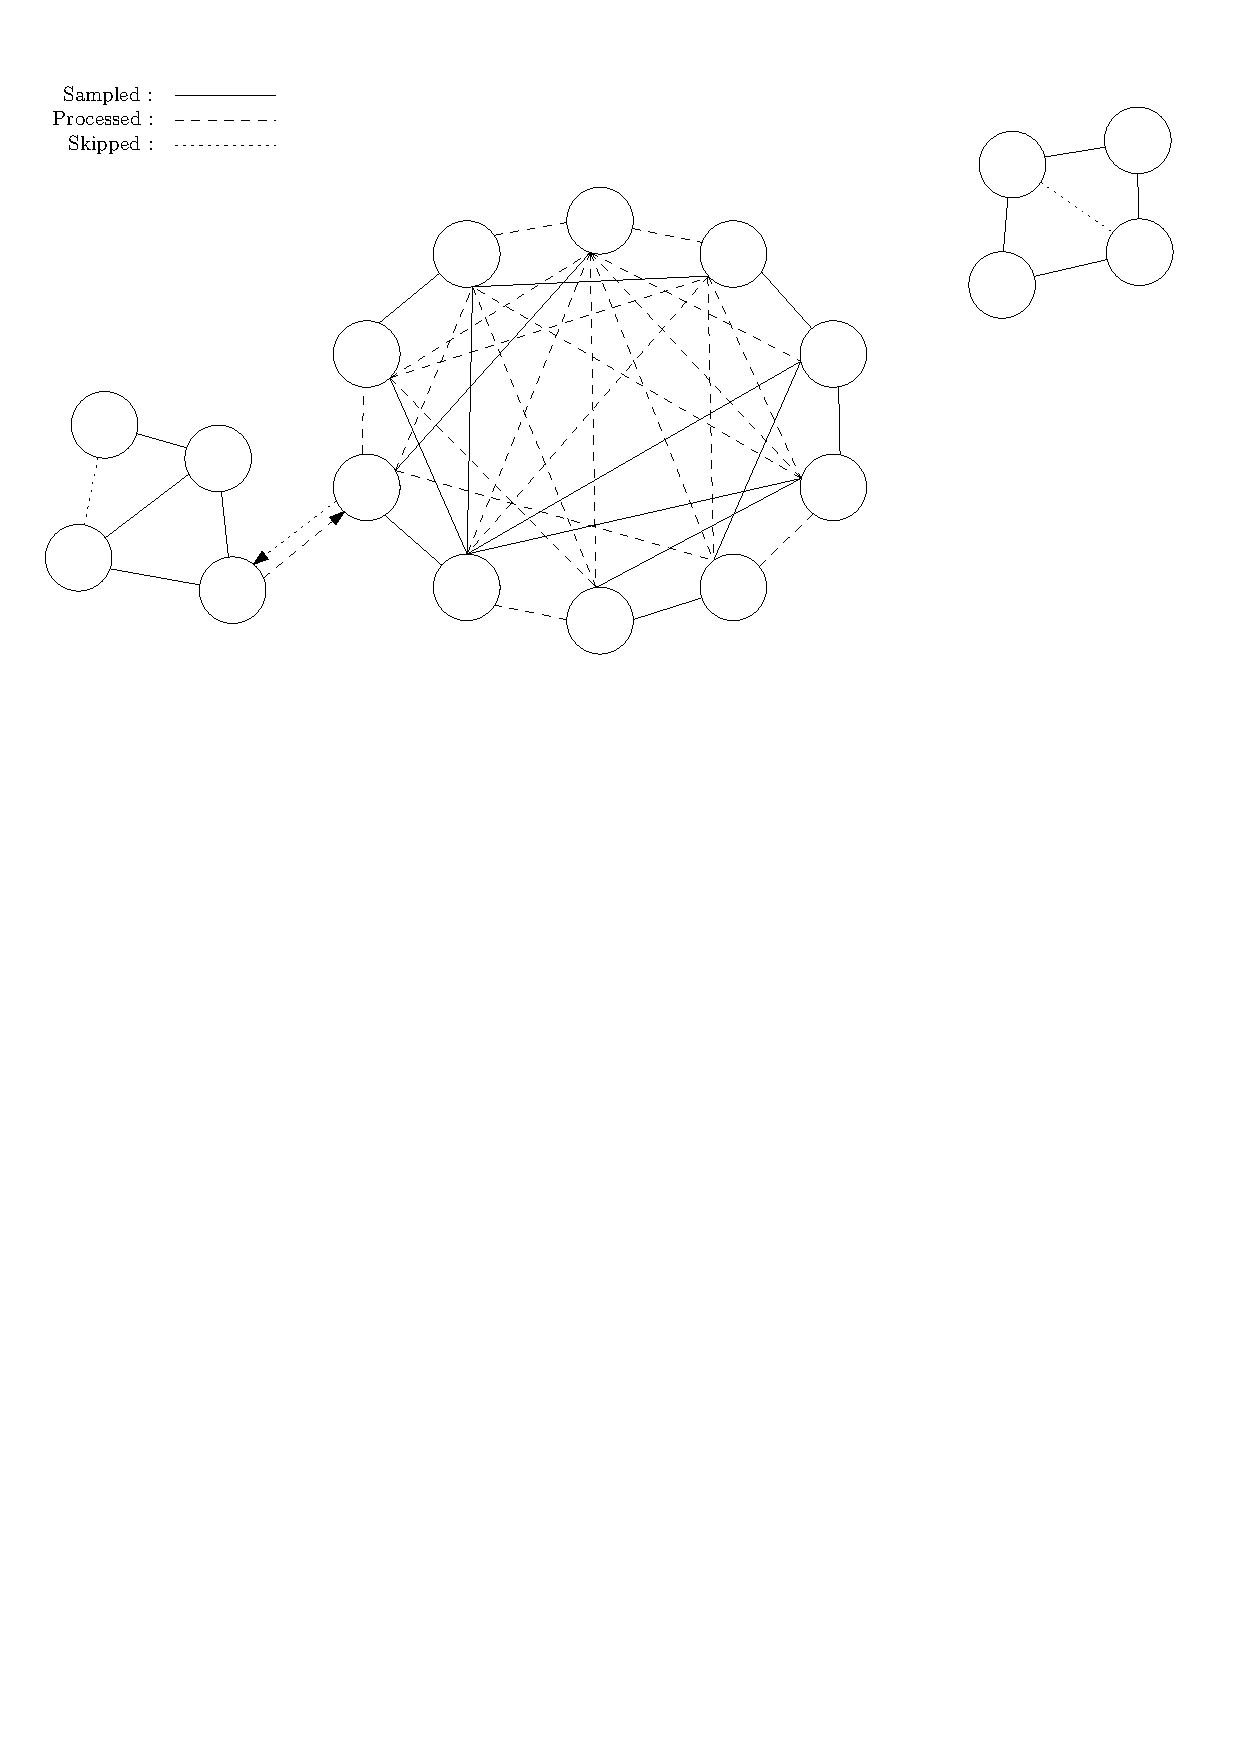
\includegraphics[width=7cm]{fig-4} }%
    \caption{Component skip : where we skip edges in the largest component, and process the rest of the graph}
    \label{fig-skip}%
\end{figure}
\paragraph{}
The general reason sampling might be a good idea comes from from the work seen in Frieze et al.[61].
Frieze et al. showed that given a d-regular graph $G$, and a subset of the graph $G'$ or the sampled graph they showed that by sampling edges with $p \ge \frac{\alpha}{d}$ for some $\alpha > 1$, then $G'$ contains a component of size $\Theta(|V|)$. 

\paragraph{}
By doing so we can prove that the expected number of edges in $G'$ is $O(|V|)$.
By defenition of $G$ $|E| = \frac{d}{2}|V|$. Each edge is sampled with probility $p=\frac{\alpha}{d}$, then the expected number of edges in $G'$ is $p\cdot |E| = \frac{\alpha}{2} = O(n)$. This can be generalized to multiple component regular $d$ graphs such that we still obtain the same $O(n)$ bound on the sample size. 

\paragraph{}
We note that this does not generalize to none d-regular graphs, but gives us an opertunity to apply a type of model onto the problem. Furthermore, unifomily sampling from $G$ creates a bais towards verticies with with high degree. Instead, we sample on neigbourhood basis such that the number of edges we sample in the neigbourhood of $v$ have probility of $\frac{\alpha}{|N(v)|}$, such that $N(v)$ is the neighbourhood of vertex $v$. If our graph is d-regular, then the proof still applies.

\paragraph{}
We now present the afforest algorithm in algorithm 3. We first obtain a sample graph, by sampling a number of rounds. We then compress all the nodes to depth one, and find the most frequent component in our sample. We then skip any vertex in our sample, and process the remaining edges. With everything discused above, this results in every vertex knowing which component it belongs in. A key different of our algorithm compared to the algorithm provided by Michael Sutton et al.[1] is that we perform our compress after sampling the graph allowing us to perform all sampling in parrallel.


\begin{algorithm}
\caption{Link Operation}\label{euclid}
\begin{algorithmic}[1]
\Procedure{Afforest}{$V,E,\textit{rounds}$}

\For{$v \in V$}
\State $\pi(v) \gets v$
\EndFor

\For{$i \gets 1 $ \textbf{to} \textit{rounds} }
  \For{$\{v\in V : i \le |N(v)|\}$}
  \State $link(v,N_i(v),\pi)$
  \EndFor
\EndFor


\For{$v \in V$}
\State $compress(v,\pi)$
\EndFor
\State $c = most\_frequent\_element(\pi)$

\For{$\{v\in V : \pi(v) \neq c\} $}
  \For{$\{v\in V : rounds + 1 \le i \le |N(v)|\}$}
  \State $link(v,N_i(v),\pi)$
  \EndFor
\EndFor


\For{$v \in V$}
\State $compress(v,\pi)$
\EndFor

\Return $\pi$
\EndProcedure
\end{algorithmic}
\end{algorithm}

\paragraph{}
There was one detail in the original paper by Michael Sutton et al.[1] where they mention that finding the most freqent element is easily obtained with random sampling. However, we could not find any research which indicated this thus we shall prove that with a delta between the most frequent element, and the second most freqent element, we can calculate an upperbound on the number of samples needed for finding the most frequent element.

\paragraph{}
Let $X_1$ be the number of elements in our sample containing the most frequent element.
Let $X_2$ be the number of elements in our sample containing the second most frequent element.
Let $m_i$ be the number of elements in a set pretaining to the $i$th most frequent element, $k$ be the total number of samples chosen, and $n$ the total population.
Then if we use random indicator varible with (1 : an element is in sample, and 0 otherwise); we get and expected value of $E(X_i) = k\frac{m_i}{n} = kf_i$, such that $f_i$ is the frequency of the $i$th  most frequent element.

\paragraph{}
If we took a $k$ size sample of elements and choose them most frequent element. Then what we are looking for is the probility that $X=X_1-X_2 \ge 0$, since $X_1 \ge X_2 \ge ... \ge X_l$. 
Furthermore, due to linartiy of expectation $E(X)=E(X_1-X_2) = E(X_1)-E(X_2) = k(f_1-f_2)$.
Since we are dealing with a binomial distribution, we can use a chernoff bound, which is an overapproximation of the taylor series of the binomial distribution.
$$P(X\le(1-\sigma)\mu) \le \exp(-\frac{\sigma^2 u}{2}) \textit{ for } 1 \le \mu \le 0$$

\paragraph{}
Where $\sigma$ is a value that we choose to obtain the tail end of a distribution, and $\mu$ is the expected value of our random vairble.
If we choose a $\sigma = 1$ then we obtain the following formula:
$$P(X\le 0) \le \exp(-\frac{u}{2})$$
We also want to find values when $X\ge 0$ so we solve for the following :
\begin{align*}
  1 - P(X\le 0) \ge& 1 - \exp(-\frac{u}{2})\\
  P(X_1-X_2 \ge 0) \ge& 1 - \exp(-\frac{k(f_1-f_2)}{2})\\
  k \ge& \frac{-2(1-P(X\ge 0))}{(f_1-f_2)}
\end{align*}
Therefore, within a certain delta frequency we can always calculate the most frequent element in constant time with probility $0<p<1$. If we look at table \ref{tab-freq} we see the exact calculations.

\begin{table}[H]
\centering
\begin{tabular}{|l|l|l|}
\hline
\multicolumn{1}{|c|}{\textbf{P(X\textgreater{}0)}} & \multicolumn{1}{c|}{\textbf{f1-f2}} & \multicolumn{1}{c|}{\textbf{k}} \\ \hline
0.9999                                             & 0.01                                & 1842                            \\ \hline
0.9999                                             & 0.02                                & 921                             \\ \hline
0.9999                                             & 0.05                                & 368                             \\ \hline
0.9999                                             & 0.1                                 & 184                             \\ \hline
0.9999                                             & 0.2                                 & 92                              \\ \hline
0.9999                                             & 0.4                                 & 46                              \\ \hline
0.9999                                             & 0.5                                 & 37                              \\ \hline
0.9999                                             & 0.7                                 & 26                              \\ \hline
0.9999                                             & 0.9                                 & 20                              \\ \hline
0.9999                                             & 1                                   & 18                              \\ \hline
\end{tabular}
\caption{Showing the sample size needed for each difference in frequency for the worst case}
\label{tab-freq}
\end{table}
\section{Analysis}
At the core, afforest is composed of two main procedures : link, and compress. The amount of sequential work that these procedures do is propotinal to the height of their trees.
\section{Implementaiton Details}

\paragraph{}
In Afforest the number of rounds that we choose to sample was $2$ since it satisfies the property that $\alpha > 1$.
For the most frequent element we choose a sample size of approximily 2000 as that gave a probility of 0.9999 for a delta frequency of 0.01 for the most frequent element, and the second most freqent element.
If you know a close approximation for the size of the component, on can always use the specified above to calculate the sample size.
Used OpenMp for our as our work stealing scheduler for scheduling threads.
Furthermore we used C++ standard library atomic header for compare and swap opeations, as well as memory access paterens.
The graph we used was a USA roadmap with approxily 90\% connectivity.
We used a machine with 32 cores, and 64 threads which ran an Intel Broadwell 2697Av4 at 2.6Ghz.


 - how does afforest work\\
 - what is the underlying data-structure for afforest (forest)\\
 - compare and swap operation (what it does, pros, cons)\\
 - link operation\\
 - Case A : in a connected component\\
 - Case B : not in a connected component\\
 - any modification does not modify previous ancestors (point out that this can\\ become a bottle neck to the algorithm)
 - compress operation\\
 - show that any compress operation results in a degree 1 tree\\
 - any race condition results in a shorter path\\
 - expected height of the tree\\
 - union find analysis (incremental randomization) \\
 - probability that it will deviate \\
 - further improvement : parallel find head of linked list\\
 - d-regular graphs\\
 - techniques that they use to sample (edge sample vs neighbour sample)\\
 - problem with generalization of\\
 - Why we want to sample our graph\\
 - How the lemma above kinda explains our goal\\
 - display algorithm and explain each step
 - finding most frequent element (proof) (not well explained in paper)\\
 - explain algorithm complexity :\\
    - worst case\\
    - expected case\\
    - best case\\
- improvements on the algorithm (use a find linked list head)\\
 
 
 
 \section*{Implementation Details}
 - how is the forest represented\\
 - how is the graph stored\\
 - how do we choose our sample\\
 
 \section{Experimental Evaluation}
 - running time
 - speed up compared with no random sampling
 - [implement thread distribution running time]
 
 \section{Improvements}
 - how do we reduce the number of CAS operations (since they are expensize)
  - on method could be to go up the entire tree (if two items are in the same component then we don't change a path)
  - downside (we need to traverse more of the tree)
  - find a fast parallel pointer jumping algorithm for multiple lists
  - downside (if we did this we are looking for a path of size logn, in a pool of lists of size n)
 
 \section{Conclusions}
 \section{Bibliography}
 \begin{verbatim}
 [1]https://ieeexplore-ieee-org.proxy.library.carleton.ca/document/8425156/references#references
 [2]https://ieeexplore-ieee-org.proxy.library.carleton.ca/document/6877288/references#references
 [3]https://dl-acm-org.proxy.library.carleton.ca/citation.cfm?id=2733089
 [4]https://www-sciencedirect-com.proxy.library.carleton.ca/science/article/pii/0196677482900086
 [5]https://dl-acm-org.proxy.library.carleton.ca/citation.cfm?id=2612692
 [6]https://link.springer.com/chapter/10.1007/3-540-45591-4_68
 [7]http://diestel-graph-theory.com/index.html
 [8]https://dl-acm-org.proxy.library.carleton.ca/citation.cfm?id=234534 
 [9]https://dl-acm-org.proxy.library.carleton.ca/citation.cfm?id=331608
 [10]https://dl-acm-org.proxy.library.carleton.ca/citation.cfm?id=3210393
 [11]https://dl.acm.org/citation.cfm?id=263872
 [12]https://link.springer.com/chapter/10.1007/978-0-8176-4842-8_15
 [13]https://dl.acm.org/citation.cfm?id=1942094
 [14]https://dl.acm.org/citation.cfm?doid=362248.362272
 [15]https://dl.acm.org/citation.cfm?id=2503246
 [16]https://ieeexplore.ieee.org/document/4569669
 [17]https://dl.acm.org/citation.cfm?id=550359
 [18]https://www.sciencedirect.com/science/article/pii/0898122181900080
 [19]https://www.sciencedirect.com/science/article/pii/0020019085900249
 [20]https://dl.acm.org/citation.cfm?id=663154
 [21]https://dl.acm.org/citation.cfm?id=362272
 [22]https://dl.acm.org/citation.cfm?id=322235
 [23]https://www.sciencedirect.com/science/article/pii/0020019082901314
 [24]https://dl-acm-org.proxy.library.carleton.ca/citation.cfm?id=739745
 [25]https://dl-acm-org.proxy.library.carleton.ca/citation.cfm?id=305744
 [26]https://dl-acm-org.proxy.library.carleton.ca/citation.cfm?id=254195
 [27]https://dl-acm-org.proxy.library.carleton.ca/citation.cfm?id=182530
 [28]https://dl-acm-org.proxy.library.carleton.ca/citation.cfm?id=359141
 [29]https://dl-acm-org.proxy.library.carleton.ca/citation.cfm?id=214077
 [30]https://dl-acm-org.proxy.library.carleton.ca/citation.cfm?id=106163
 [31]https://dl-acm-org.proxy.library.carleton.ca/citation.cfm?id=203622
 [32]https://dl-acm-org.proxy.library.carleton.ca/citation.cfm?id=358650
 [33]https://dl-acm-org.proxy.library.carleton.ca/citation.cfm?id=72952
 [34]https://dl-acm-org.proxy.library.carleton.ca/citation.cfm?id=586952
 [35]https://dl-acm-org.proxy.library.carleton.ca/citation.cfm?id=1398907
 [36]https://www.sciencedirect.com/science/article/pii/0166218X84900192
 [37]B. Awerbuch and Y. Shiloach. New connectivity and MSF algorithms for Ultracomputer and PRAM. In ICPP, pages 177--187, 1983.
 [38]https://dl-acm-org.proxy.library.carleton.ca/citation.cfm?id=237563
 [39]https://dl-acm-org.proxy.library.carleton.ca/citation.cfm?id=123143
 [40]https://dl-acm-org.proxy.library.carleton.ca/citation.cfm?id=247524
 [41]https://dl-acm-org.proxy.library.carleton.ca/citation.cfm?id=377897
 [42]https://dl-acm-org.proxy.library.carleton.ca/citation.cfm?id=586952
 [43]https://dl-acm-org.proxy.library.carleton.ca/citation.cfm?id=686427
 [44]S. Hambrusch and L. TeWinkel. A study of connected component labeling algorithms on the MPP. In Supercomputing, pages 477--483, 1988.
 [45]S. Goddard, S. Kumar, and J. F. Prins. Connected components algorithms for mesh-connected parallel computers. In Parallel Algorithms: 3rd DIMACS Implementation Challenge, pages 43--58, 1995.
 [46]T.-S. Hsu, V. Ramachandran, and N. Dean. Parallel implementation of algorithms for finding connected components in graphs, 1997
 [47]https://dl-acm-org.proxy.library.carleton.ca/citation.cfm?id=1196220
 [48]https://dl-acm-org.proxy.library.carleton.ca/citation.cfm?id=1079430
 [49]https://dl-acm-org.proxy.library.carleton.ca/citation.cfm?id=2358680
 [50]https://dl-acm-org.proxy.library.carleton.ca/citation.cfm?id=2312018
 [51]https://dl-acm-org.proxy.library.carleton.ca/citation.cfm?id=746654
 [53]A. Krishnamurthy, S. S. Lumetta, D. E. Culler, and K. Yelick. Connected components on distributed memory machines. In Parallel Algorithms: 3rd DIMACS Implementation Challenge, pages 1--21, 1994.
 [54]https://dl-acm-org.proxy.library.carleton.ca/citation.cfm?id=231641
 [55]E. Caceres, H. Mongelli, C. Nishibe, and S. W. Song. Experimental results of a coarse-grained parallel algorithm for spanning tree and connected components. In High Performance Computing & Simulation, pages 631--637, 2010.
 [56]https://dl-acm-org.proxy.library.carleton.ca/citation.cfm?id=1869229
 [57]J. Soman, K. Kishore, and P. J. Narayanan. A fast GPU algorithm for graph connectivity. In IPDPS, pages 1--8, 2010.
 [58]https://dl-acm-org.proxy.library.carleton.ca/citation.cfm?id=2192614
 [59]https://dl.acm.org/citation.cfm?id=2059488
 [60]https://www.ams.org/journals/proc/1956-007-01/S0002-9939-1956-0078686-7/home.html
 [61]https://arxiv.org/abs/1605.06643
  \end{verbatim}


\end{document}
